\documentclass[../../main.tex]{subfiles}
\DeclareSIUnit{\arbunits}{[arb.u.]}

\begin{document}

    Zur Messung der Charakteristik des verwendeten Radioteleskops werden Spektren der Sonnen aufgenommen. Dabei wird die Sonne als punktförmige Lichtquelle betrachtet. Das ist hier möglich, da die Ausdehnung der Sonne am Erdhimmel viel kleiner als die Winkelauflösung des Teleskops ist. Für die Messung wird der Signal-Modus vewendet. So lässt sich später eine Aussage über die absolute Intensität der Spektren treffen. Da für die Messung die Intensität der Sonnenstrahlung von Interesse ist, wird die Messfrequenz um \SI{10}{\mega \hertz} nach unten aud \SI{1410,40}{\mega \hertz} korrigiert. Das führt dazu, dass die Wasserstofflinien, die aus extrasolaren Quellen stammen, nicht mehr aufgenommen werden. Dies ist notwendig, da die Wasserstofflinien das Ergebnis sonst verfälschen. Die Bandbreite der Messung wurde auf \SI{2}{\mega \hertz}, die Frequenzauflösung auf \SI{7,8}{\mega \hertz} und die Anzahl an Kanälen auf 256 eingestellt. Die Integrationszeit, also die Zeit über der das Spektrum aufgenommen wird, beträgt \SI{10}{\second}. Vergleichbar ist diese Zeit mit der Belichtungszeit einer Fotokamera. \\
    Bei der ersten Messreihe, wird das Umfeld der Sonne mit einem Gitter abgerastert. Die Sonne erreicht in Onsala am Messtag (31.01.2024) mittags nur eine Höhe von ca. \ang{15} über dem Horizont. Das ist weniger als die für die Messung erforderten \ang{20}. Allerdings ist die Strahlung der Sonne so stark, dass diese auch bei niedrigeren Winkeln gemessen werden kann. Für eine gute Messung sollte die Höhe von \ang{10} über dem Horizont nicht unterschritten werden. Deshalb werden zwei Gitter abgerastert. Relativ zur Position der Sonne für Azimuthwinkel von \ang{-10} bis \ang{+10} und Höhenwinkel von \ang{0} bis \ang{10} mit 15 Messpunkten und ein weiteres Gitter für Azimuthwinkel von \ang{-7.5} bis \ang{+7.5} und Höhenwinkel von \ang{-2.5} bis \ang{7.5} mit 12 Messpunkten. Die Abstände zwischen den einzelnen Messpunkten im jeweiligen Gitter beträgt \ang{5}.
    Für die weitere Beobachtung wird ein Kreuzscan durch die Sonne durchgeführt. Dabei wird der Azimuthwinkel bei festem Höhenwinkel von \ang{0} in \ang{2}-Schrtten von \ang{-16} bis \ang{+16} variiert. In der Höhenrichtung wird dies für einen festen Azimuthwinkel von \ang{0} bei einem Höhenwinkel von \ang{-4} bis \ang{-16} in \ang{1}-Schritten durchgeführt.
    In \autoref{fig:TT:SonneSpektrum00} ist ein Beispiel für das Sonnenspektrum gezeigt. Dieses ist theoretisch genau auf die Sonnen aufgerichtet aufgenommen worden. Es handelt sich um die unnormierte absolute Intensität der Sonnenstrahlung. Aufgrund der fehlenden Normierung können die Werte der aufgenommen Spektren zwar untereinander verglichen werden, nicht aber mit anderen Messungen an anderen Aufbauten. Die Intensität ist deshalb in willkürlichen Einheiten (arb. u.) angegeben. Auf der X-Achse ist die Relativgeschwindigkeit relativ zum LSR (Local standard of Rest) angegeben. Bei der Verschiebung der Messfrequenz um \SI{10}{\mega \hertz}, entspricht das bei einer Bandbreite von \SI{2}{\mega \hertz} gerade dem Bereich von ca. \SI{1800}{\mega \hertz} bis \SI{2400}{\mega \hertz}. Für die Bestimmung der Gesamtintensität des Spektrums wird von \SI{1950}{\kilo \metre \per \second} bis \SI{2300}{\kilo \metre \per \second} integriert. Dies wird bei jedem Spektrum gleich gehandhabt, um so eine Vergleichbarkeit zu erhalten.
    \begin{figure}[H]
        \centering
        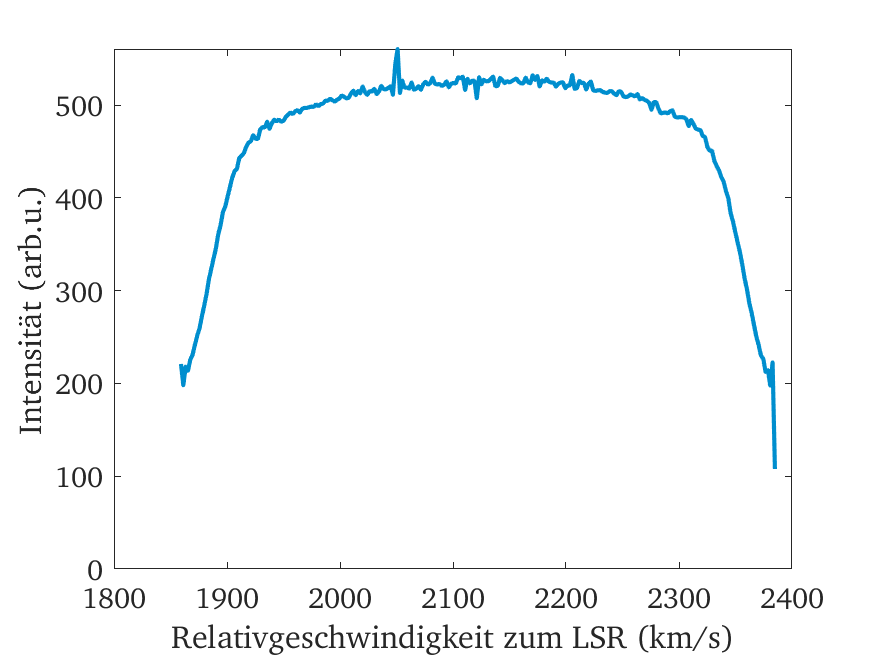
\includegraphics[width=0.75\textwidth]{Bilddateien/Sun/Raster_spectrum_64867__Fig_1.png}
        \caption{Spektrum der Messung der Sonnenintensität bei einem zur Sonne relativen Azimuthalwinkel von \ang{0} und einem Höhenwinkel von \ang{0}.}
        \label{fig:TT:SonneSpektrum00}
    \end{figure}
    Die so ermittelten Intensitäten aus den Beispielspektren sind in \autoref{fig:TT:SonneInterpolationMap} abgebildet. Die Daten wurden dabei interpoliert, um eine bessere Übersicht zu erhalten. Dabei wurden alle verfügbaren Intensitäten aus der Raster- und der Kreuzmessung berücksichtigt. Für die Darstellung der interpolierten Daten wurde der Bereich der Rastermessung gewählt, da hier eine ausreichende Anzahl an Daten vorliegt, um valide Aussagen treffen zu können. Des Weiteren reicht dieser Bereich aus, um die Aussagen über die Signalverschiebung des Teleskops zu treffen.
    \begin{figure}[H]
        \centering
        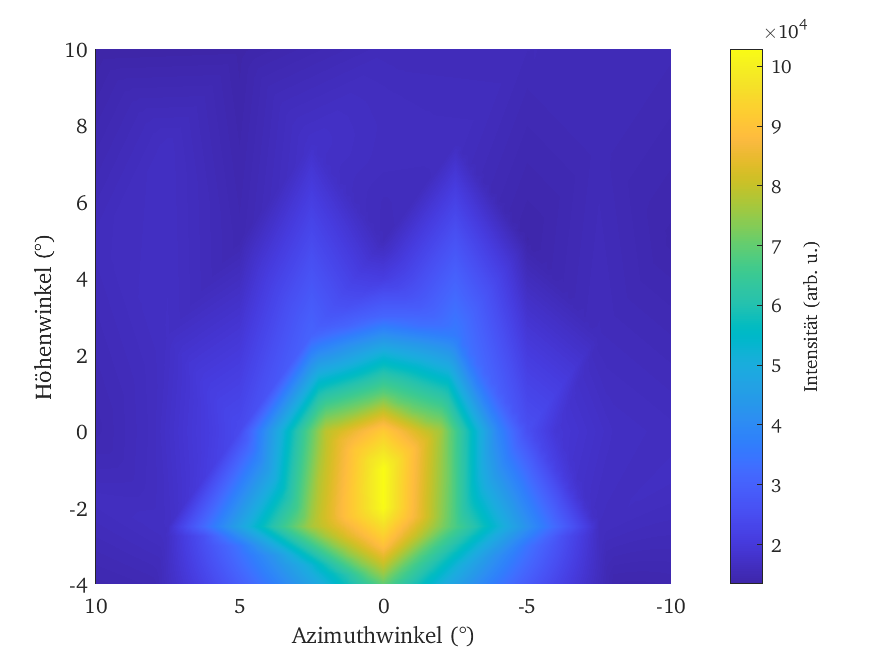
\includegraphics[width=\textwidth]{Bilddateien/Sun/Raster_Map_Fig_1011.png}
        \caption{Interpolierte Daten aus den Intensitätsmessungen. Als Datengrundlage dient hier sowohl der Kreuzscan, als auch die Rastermessung. Die Daten sind nur im Bereich der Rastermessung gezeigt, da hier genügend Messpunkte für eine sinnvolle Interpolation zur Verfügung stehen.}
        \label{fig:TT:SonneInterpolationMap}
    \end{figure}
    Es ist zu erkennen, dass der Intensitätspeak nicht auf dem Punkt bei 0 liegt, wo er zu vermuten wäre. Der Peak ist leicht in positiver Azimuthrichtung verschoben und liegt bei einem Azimuthwinkel von \ang{0} und einem Höhenwinkel von \ang{0} bis \ang{2}. Diese Werte sind allerdings aufgrund der Interpolation und anderen Messunsicherheiten mit einer gewissen Toleranz versehen. Eine sinnvolle Abschätzung der Unsicherheit lässt sich hier in beiden Winkelrichtungen mit \ang{+-2} angeben, womit die Kalibrierung des Teleskops für die weiteren Messungen als ausreichend angesehen werden kann. \\
    Aus der winkelabhängigen Intensistätsverteilung (\autoref{fig:TT:SonneInterpolationMap}) geht hervor, dass die Intensität der Sonne nicht in Form eines Punktes, sondern verschmiert mit einem richtungsabhängigen Gradienten erscheint. Das ist mit den Eigenschaften des Radioteleskops, bzw. dessen Antenne zu erklären. Die von der Sonne emitterten Radiowellen beugen an der Antenne des Teleskops und erzeugen somit eine Gaußverteilung des empfangenen Signals. Eine Folge der Beugung ist deshalb die Verschmierung der als punktförmig angenommen Strahlung der Sonne. Diese Verschmierung sollte gleichmäßig, also isotrop sein. Das ist nicht ganz der Fall. Hier besteht die Möglichkeit, dass weitere Umwelteinflüsse, wie z.B. die benachbarten Teleskope störend im Weg stehen. \\
    Die Gaußverteilung des Signals kann in den Intensitäten der Kreuzmessung gesehen und charakterisiert werden. In \autoref{fig:TT:SonneAzimuth} ist die Messung entlang des Azimuthwinkels aufgetragen. 
    \begin{figure}[H]
        \centering
        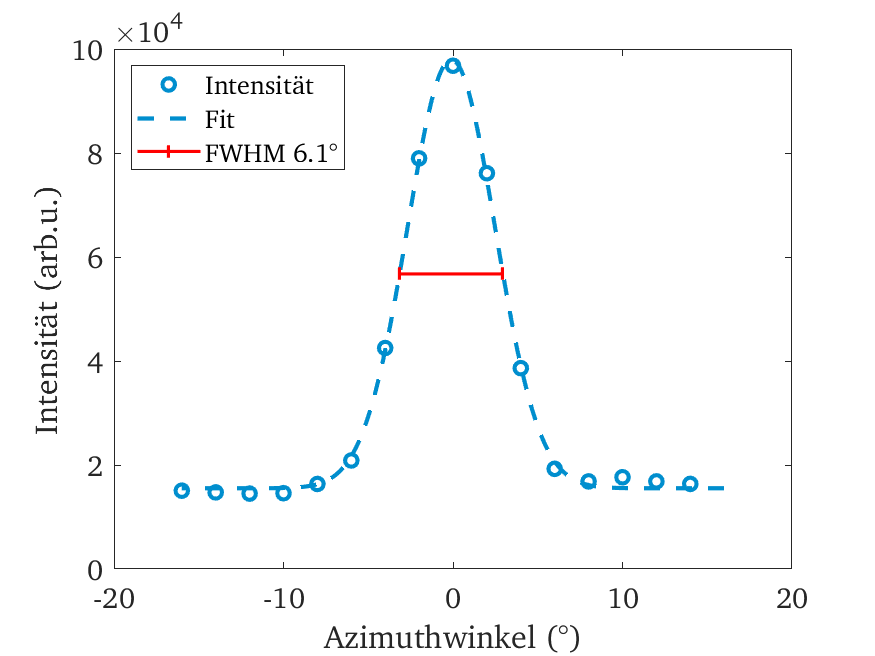
\includegraphics[width=0.75\textwidth]{Bilddateien/Sun/Kreuz_Az_FitFig_2000.png}
        \caption{Verteilung der gemessenen Intensitäten der Sonne für verschiedene Azimuthalwinkel bei einem Höhenwinkel von \ang{0}. An die Messdaten ist ein Gaußverteilung gefittet, deren FWHM bei \ang{6,1} liegt.}
        \label{fig:TT:SonneAzimuth}
    \end{figure}
    Eine Gaußfunktion mit der Vorschrift
    \begin{align*}
        f(x) = \frac{a}{w\sqrt{\frac{\pi}{2}}} \cdot \exp\left(-2\left(\frac{x-b}{w} \right)^2\right)+d
    \end{align*}
    wird an die Messdaten gefittet. Die Verschiebung auf der x-Achse lässt sich mit $b$ direkt aus den Daten des Fits ablesen. Für das FWHM (full width half maximum), also die Breite am halben Maximum, auch Halbwertsbreite genannt, muss folgende Formel angewendet werden
    \begin{align}
        \text{FWHM} = w \cdot \sqrt{2ln(2)}.
    \end{align}
    Die Unsicherheit berechnet sich mit
    \begin{align*}
        u(\text{FWHM}) = \sqrt{\left( u(w) \cdot \sqrt{2ln(2)} \right)^{2}}.
    \end{align*}
    \begin{figure}[H]
        \centering
        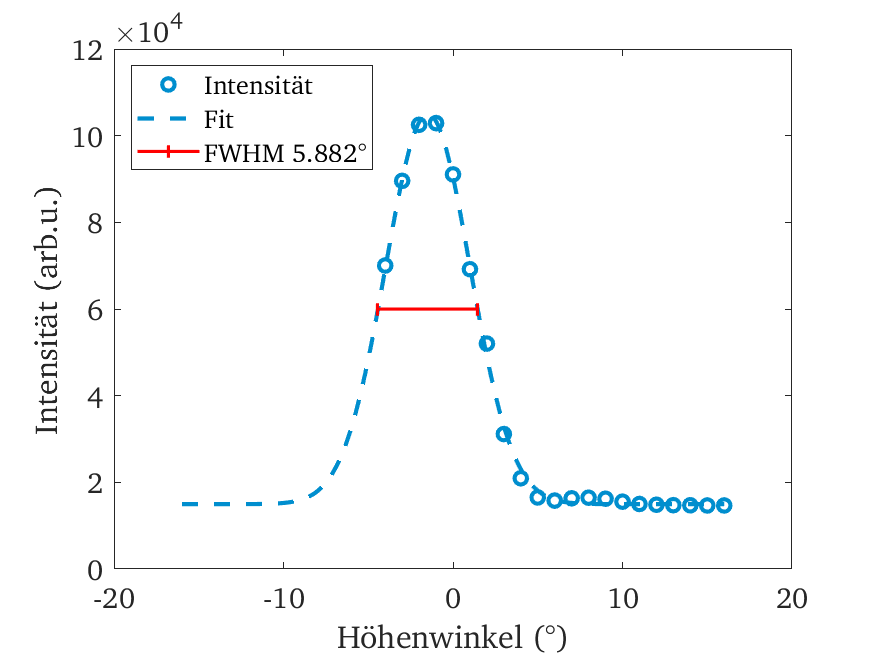
\includegraphics[width=0.75\textwidth]{Bilddateien/Sun/Kreuz_He_FitFig_3000.png}
        \caption{Verteilung der gemessenen Intensitäten der Sonne für verschiedene Höhenwinkel bei einem Azimuthalwinkel von \ang{0}. An die Messdaten ist ein Gaußverteilung gefittet, deren Halbwertsbreite (FWHM) bei \ang{5,882} liegt.}
        \label{fig:TT:SonneHöhe}
    \end{figure}
    Für die Messung in \autoref{fig:TT:SonneHöhe} bei der der Höhenwinkel variiert und der Azimuthwinkel bei \ang{0} festgehalten wurde, lässt sich auch ein Gaußfit anlegen und daraus die Parameter ableiten. Die Daten für beide Fits (Azimuthal- und Höhenmessung) sind in \autoref{tab:TT:Kreuzscan} dargestellt.
    \begin{table}[H]
        \centering
        \begin{tabular}{l|l|l|l|l|l}
        \rowcolor[HTML]{A6E1F4} 
                & $a$                                & $b$                   & $d$                                  & $w$                & FWHM               \\ \hline
        Azimuth & $\SI{5.35+- 0.18e5}{\arbunits}$ & $\ang{0.101+-0.075}$ & $\SI{1.552+- 0.084e4}{\arbunits}$ & $\ang{5.18+-0.17}$ & $\ang{6.10+-0.21}$ \\ \hline
        Höhe    & $\SI{5.64 +- 0.16e5}{\arbunits}$ & $\ang{-1.458+-0.060}$  & $\SI{1.497 +- 0.078e4}{\arbunits}$ & $\ang{5.00+-0.15}$ & $\ang{5.88+-0.18}$
        \end{tabular}
        \caption{Parameter der Fits an der Intensitätsverteilung des Kreuzscans.}
        \label{tab:TT:Kreuzscan}
    \end{table}
    Es ist deutlich zu erkennen, dass der Peak bei der Messung in der Höhenrichtung, um ca. \ang{1,5} verschoben ist. Das kann auf eine falsche Kalibrierung des Teleskops zurückzuführen sein. In der Anleitung \cite{doc:SalsaManual} ist angegeben, dass die Antenne, durch den Wind um \ang{1} bis \ang{2} verschoben werden kann. Betrachtet man die Windmessungen der Wetterstationen um Onsala findet man für den Messzeitraum (31.01.24 12:00 Uhr bis 14:00) Windböen von \SI{11,8}{\metre \per \second} bis \SI{15,4}{\metre \per \second} \cite{Wetter:WindOnsala14h}. Nach der Windwarnskala des Deutschen Wetterdienstes \cite{Wetter:Windwarnskala} entspricht das \glqq{}starkem\grqq{} bis \glqq{}steifem\grqq{} Wind. Die Versuchsanleitung geht davon aus, dass diese Windeinflüsse eine untergeordnete Rolle spielen, da die Winkelauflösung des Teleskops kleiner ist. Diese beträgt an der Halbwertsbreite (FWHM) bei \SI{1420}{\mega \hertz} ca. \ang{6} \cite{doc:SalsaManual}. Die mit den Kreuzscans ermittelten Werte $\text{FWHM}_{az}=\ang{6,10 +- 0,21}$ und $\text{FWHM}_{he}=\ang{5.88 +- 0.18}$ sind mit dieser Angabe in Übereinstimmung, auch wenn die Scans bei \SI{1410}{\mega \hertz} durchgeführt wurden.\\
    Mit Hilfe des Rayleigh-Kriteriums für Blenden \cite{dewiki:RayleighKrit} kann der Durchmesser der Teleskopantenne abgeschätzt werden. Mit dem Winkel des ersten Minimums $\alpha$, der Wellenlänge $\lambda$ und dem Blendendurchmessser (hier: Durchmesser der Antenne) $d$ gilt mit der Kleinwinkelnäherung\footnote{Hierzu muss der Winkel durch Multiplikation mit $\frac{\pi}{180}$ vom Grad- ins Bogenmaß überführt werden!}
    \begin{align}
        \alpha = 1,22 \frac{\lambda}{d}.
    \end{align}
    Dabei kann die Wellenlänge mit $\lambda = \frac{c}{f}$ aus der Frequenz $f$ bestimmt werden. Für die Unsicherheit gilt dann
    \begin{align*}
        u(d) = \sqrt{\left( u(\alpha) \cdot 1,22 \frac{c}{f \cdot \alpha^{2}} \right)^{2}}.
    \end{align*}
    $\alpha$ kann mit der Halbwertsbreite (FWHM) abgeschätzt werden. Man erhält für die beiden Messungen in Azimuthal- und Höhenrichtung die in \autoref{tab:TT:Durchmesser} gezeigten Werte.
    \begin{table}[H]
        \centering
        \begin{tabular}{l|l|l|l}
        \rowcolor[HTML]{A6E1F4} 
                & $d$                           & $t$    & $P$        \\ \hline
        Azimuth & $\SI{2.436 +- 0.084}{\metre}$ & $1,62$ & $10,96\%$ \\ \hline
        Höhe    & $\SI{2.528 +- 0.078}{\metre}$ & $2,93$ & $0,37\%$ 
        \end{tabular}
        \caption{Aus den Halbwertsbreiten ermittelte Werte für den Teleskopdurchmesser $d$. Die Abweichung vom Erwartungswert beträgt $t \cdot u(d)$. Die Übereinstimmung der Werte mit dem Literaturwert $d=\SI{2,3}{\metre}$ ist mit $P$ angegeben. }
        \label{tab:TT:Durchmesser}
    \end{table}
    Die ermittelten Werte sind im Rahmen einer Standardunsicherheit nicht mit dem Literaturwert von \SI{2,3}{\metre} \cite{doc:SalsaManual} vereinbar. Ein Signifikantest gibt eine Übereinstimmung des über die azimuthale Messung ermittelten Wertes von $10,96\%$. Bei dem über die Höhenmessung ermittelten Wert beträgt diese nur $0,37\%$. Dass der über den Azimuthalwinkel ermittelte Wert besser übereinstimmt dürfte daran liegen, dass für diesen mehr Messdaten zur Verfügung stehen, als bei der Messung über den Höhenwinkel. Die weitere Abweichung der Werte, dürfte mit den verwendeten Näherungen zusammenhängen. Allein die Kleionwinkelnäherung ist schon mit einem Fehler von bis zu $0,5\%$ versehen. Als weitere Näherung wurde verwendet, dass das erste Minimum der Halbwertsbreite entspricht. Eine Anpassung auf $\ang{6,45}$ würde den gewünschten Wert von $\SI{2,3}{\metre}$ bringen. Eine Messung bei höherem Sonnenstand (z.B. im Sommer) würde möglicherweise bessere Ergebnisse liefern. Auch die Messung an einem windstillen Tag wäre zu empfehlen.

    \subsubsection{Einfluss des Messmodus}
        Im Folgenden soll kurz auf die beiden Messmodi \glqq{}switched mode\grqq{} und \glqq{}signal mode\grqq{} eingegangen werden.
        \begin{figure}[H]
            \centering
            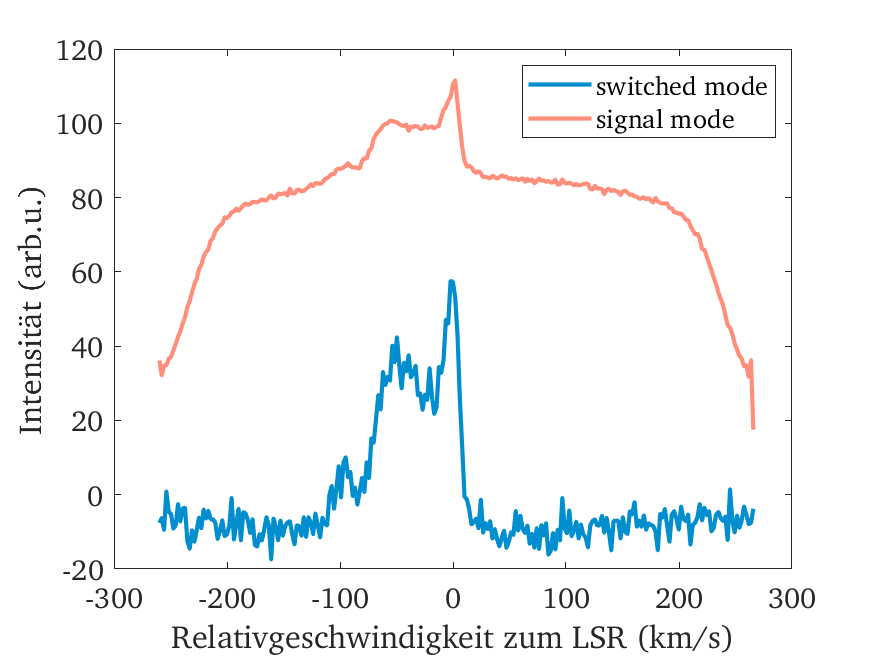
\includegraphics[width=0.75\textwidth]{Bilddateien/Modi/Fig_10.png}
            \caption{}
            \label{fig:TT:MessModi}
        \end{figure}
        In \autoref{fig:TT:MessModi} werden die Messmodi verglichen. Dabei wird das selbe Objekt angefahren und eine Messung bei $\SI{1420}{\mega \hertz}$ durchgeführt. Es ist zu erkennen, dass im \glqq{}switched mode\grqq{} der Hintergrund vom Messsignal abgezogen wird. Das geschieht in dem bei einer etwas höheren Frequenz ein zweites Spektrum aufgenommen und von der Messung bei $\SI{1420}{\mega \hertz}$ abgezogen wird. Bei dieser Methode wird davon ausgegangen, dass die Hintergrundintensität aus der Charakteristik der Antenne stammt und keine weiteren Quellen hat. Da die Intensität im \glqq{}switched mode\grqq{} ins negative geht, ist zu erkennen, dass diese Annahme nicht vollständig zutrifft. Für die Messung der Relativgeschwindigkeiten der Milchstraße, die im folgenden Abschnitt ausgewertet werden, ist die absolute Intensität allerdings nicht von Interesse. Für diese Messung, ist es wichtig die Positionen der Peaks auf der x-Achse erkennen zu können. Dazu muss lediglich das Verhältnis von Peaksignal zum Hintergrund genügend groß sein, was mit der Methode des \glqq{}switched mode\grqq{} gut funktioniert. 
    
\end{document}